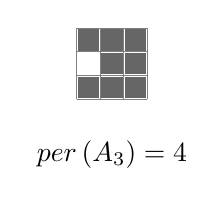
\begin{tikzpicture}
\draw[step=0.3cm,gray,thin] (0,0) grid (0.8999999999999999,0.8999999999999999);
\fill[black!60!white] (0.015,0.885) rectangle (0.285,0.6149999999999999);
\fill[black!60!white] (0.315,0.885) rectangle (0.585,0.6149999999999999);
\fill[black!60!white] (0.6149999999999999,0.885) rectangle (0.885,0.6149999999999999);
\fill[black!60!white] (0.315,0.585) rectangle (0.585,0.315);
\fill[black!60!white] (0.6149999999999999,0.585) rectangle (0.885,0.315);
\fill[black!60!white] (0.015,0.285) rectangle (0.285,0.015000000000000013);
\fill[black!60!white] (0.315,0.285) rectangle (0.585,0.015000000000000013);
\fill[black!60!white] (0.6149999999999999,0.285) rectangle (0.885,0.015000000000000013);
\node[] at (0.44999999999999996,-0.7) {  $\text{per}\left(A_{3}\right)=4$};\end{tikzpicture}